\RequirePackage{silence}
\documentclass[10pt, compress,british,xcolor={svgnames,dvipsnames,x11names},trans]{beamer}

\usepackage[english]{babel}
\usepackage[utf8]{inputenc}
\usepackage{csquotes}
\usepackage{comment}
\usepackage{tikzsymbols}

\definecolor{darkgreen}{rgb}{0.0, 0.5, 0.0}
\def\area#1{{\color{darkgreen}area:\it #1}}
\def\food#1#2{{Dial. state #1: \color{blue}food:\it #2}}
\def\pricerange#1{{\color{orange}pricerange:\it #1}}
\def\sys#1{{\color{purple}System: \it #1}}
\def\usr#1{{\color{brown}User: \it #1}}
\def\api#1{{\color{blue}DB annotations: \it #1}}

% OP - Ondrej Platek inline 
\definecolor{purple}{RGB}{200,0,200}
\def\OP#1{{\color{purple}OP: \it #1}}
\def\OPdel#1{\bgroup\markoverwith{\textcolor{purple}{\rule[0.5ex]{2pt}{1pt}}}\ULon{#1}}


\usepackage{eso-pic}
\beamertemplatenavigationsymbolsempty
\newcommand\AtPagemyUpperLeft[1]{\AtPageLowerLeft{%
\put(\LenToUnit{0.91\paperwidth},\LenToUnit{0.915\paperheight}){#1}}}
\AddToShipoutPictureFG{
  \AtPagemyUpperLeft{{
\includegraphics[width=.8cm,keepaspectratio]{logo_ufal_165.png}}}
}%


%%% mtheme customisations
% \usetheme[frametitleformat=regular,progressbar=frametitle,block=fill]{m}
\usetheme[progressbar=frametitle]{m}
\AtBeginSubsection{
\metroset{color/background=dark}
\frame[plain,c]{
  \begin{center}
  \begin{minipage}{25em}
    \usebeamercolor[fg]{section title}
    \usebeamerfont{section title}
    \insertsubsection\\[-1ex]
    \usebeamertemplate*{progress bar in section page}
  \end{minipage}
  \end{center}
}
\metroset{color/background=light}
}
%%%%% end mtheme

\setbeamertemplate{frametitle continuation}[from second]
\setbeamertemplate{bibliography item}[book]

\usetikzlibrary{arrows}
\usetikzlibrary{chains}
\usepackage{tikz-qtree}
\usepackage{multicol}


\usepackage{expex}
%\lingset{glhangindent=2em,glspace=1em,aboveexskip=0pt,belowexskip=0pt,aboveglftskip=-3pt,extraglskip=3pt} %v0.1
%\lingset{exskip=0pt,interpartskip=-3pt,belowpreambleskip=-3pt,belowglpreambleskip=-3pt,aboveglftskip=-3pt,extraglskip=3pt,glhangstyle=none}
\usepackage{relsize}
\usepackage{booktabs,tabularx}
%\usepackage{textcomp}
\usepackage{listings}
\lstset{basicstyle=\ttfamily,breaklines=true,breakatwhitespace=true,
keywordstyle={\color{NavyBlue}\bfseries}, showstringspaces=false,
commentstyle={\color{PaleVioletRed4}},
emphstyle={\color{OliveGreen}\bfseries}
}

\usepackage{algorithmic}
\renewcommand{\algorithmiccomment}[1]{\alert{/* #1 */}}

\usetikzlibrary{shapes.multipart}
\usetikzlibrary{positioning}
\usetikzlibrary{arrows.meta}

\makeatletter
\pgfarrowsdeclare{crow's foot}{crow's foot}
{
  \pgfarrowsleftextend{+-.5\pgflinewidth}%
  \pgfarrowsrightextend{+.5\pgflinewidth}%
}
{
  \pgfutil@tempdima=0.5pt%
  \advance\pgfutil@tempdima by.25\pgflinewidth%
  \pgfsetdash{}{+0pt}%
  \pgfsetmiterjoin%
  \pgfpathmoveto{\pgfqpoint{0pt}{-6\pgfutil@tempdima}}%
  \pgfpathlineto{\pgfqpoint{-6\pgfutil@tempdima}{0pt}}%
  \pgfpathlineto{\pgfqpoint{0pt}{6\pgfutil@tempdima}}%
  \pgfusepathqstroke%
}

\usepackage[os=win]{menukeys}
\usepackage{notoccite}
\usepackage[numbers,sort&compress]{natbib}


\title{{Extracting Knowledge from Dialogue}}
\subtitle{Ph.D. Thesis Proposal}
\titlegraphic{logo_ufal_165.png}


\author{{\bf Ondřej Plátek} \\ \footnotesize{\texttt{oplatek@ufal.mff.cuni.cz}} \\ supervisor: {\bf Ing. Mgr. Filip Jurčíček, Ph.D.} }
\institute{
Institute of Formal and Applied Linguistics\\
Faculty of Mathematics and Physics\\
Charles University in Prague
}

\begin{document}

\maketitle


\section{Task description}  %%%%%%%%%%%%%%%%%%%%%%%%%%%%%%%%%%%%%%%%%%%%%%%%%%%%%%%%%%%%%%%%


\begin{frame}\frametitle{Narrow domain task oriented dialogues}
    {\bf User's goal: {\it food="chinese", area="city center"}} \\
    \vfill
    \sys{Hello, welcome to the Cambridge restaurant system! \dots } \\
    \usr{I would like a Chinese restaurant} \\
    \sys{A golden house is a Chinese restaurant in the city center} \\
    \dots

    \begin{itemize}
        \item {\bf Narrow restaurant domain}~\cite{henderson2014second} $\longrightarrow$ targeted semantics
        \item {\bf Task oriented} $\longrightarrow$ system provides information from database (DB)
        \item {\bf Turn based} $\longrightarrow$ user marks end of turn \& easier annotations
        \item {\bf Goal: shallow semantics} $\longrightarrow$ able to answer most frequent types of user questions with a help of DB
            \begin{itemize}
                \item Cooperative user $\longrightarrow$ no reasoning about sensibility of users input   
                \item {\color{darkgreen} Out-of-domain and out-of-application requests~\cite{bohus_thesis} with no special treatment} $\longrightarrow$ {\color{red} {\bf future work}}
            \end{itemize}
    \end{itemize}
\end{frame}

\begin{frame}\frametitle{Optimizing end-to-end text-to-text dialogue}
    \begin{itemize}
        \item {\bf Text-to-text} $\longrightarrow$ single modality (extensible to speech)
        \item {\bf End-to-end single model architecture} $\longrightarrow$ principled approach
            \begin{itemize}
                \item {\bf Less annotations $\longrightarrow$ easier data collection}
                \item No cumulation of errors in pipeline
                \item Implicitly able to model properties which used to be handcrafted 
                \begin{itemize}
                    \item Entrainment
                    \item Dialogue state update - coreference resolution
                \end{itemize}
            \end{itemize}
    \end{itemize}
\end{frame}

% TODO do not show bullet points at the first level - different colour
\begin{frame}\frametitle{Challenges}
    % \begin{itemize}
        % \item 
            {\bf \color{blue} Reply generation} given dialogue history
            \\
            \begin{itemize}
                \item Language variability, ambiguity, long context, \dots
            \end{itemize}
        % \item 
            {\bf \color{blue} Conditioning on database} when generating reply
            \\
            \begin{itemize}
                \item Representing structured knowledge in statistical models
            \end{itemize}
        % \item 
            {\bf \color{blue} Datasets}
            \\
            \begin{itemize}
                \item Even narrow-domain  dialogue has huge branching factor
                \item Narrow domain $\longrightarrow$ lack of data
                \item Each new domain has to {\bf collect specific bootstrap data}
            \end{itemize}
        % \item 
            {\bf \color{blue} Lack of evaluation metrics} for dialogue response generation
            \\
            \begin{itemize}
                \item Datasets too small $\longrightarrow$ {\bf supervised feedback not convenient}
                \item Task completions~\cite{todo}, appropriateness~\cite{todo}, \dots 
                \begin{itemize}
                    \item {\bf Weak and noisy} reinforcement {\bf signals}
                \end{itemize}
            \end{itemize}
    % \end{itemize}
\end{frame}

\begin{frame}{Table of contents}
  \setbeamertemplate{section in toc}[sections numbered]
  \tableofcontents[hideallsubsections]
\end{frame}


\section{Motivation}  %%%%%%%%%%%%%%%%%%%%%%%%%%%%%%%%%%%%%%%%%%%%%%%%%%%%%%%%%%%%%%%%

\begin{frame}\frametitle{End-to-end optimized task-oriented dialogue systems}
\begin{columns}
\begin{column}{0.45\textwidth}
    {\bf Current state} \\
    \begin{itemize}
        \item Multiple components
            \begin{itemize}
                \item Often handcrafted
                \item LU, DM, NLG 
            \end{itemize}
        \item Handcrafted dialogue acts
        \item Handcrafted tens of actions
            \begin{itemize}
                \item Thousands of live conversation needed for reasonable policy~\cite{gasic}
            \end{itemize}
        \item {\bf \color{red} Non trivial expert work needed for a~baseline system on new domain}
    \end{itemize}
\end{column}
\begin{column}{0.45\textwidth}
    {\bf End-to-end vs current practice}
    \begin{itemize}
        \item Single statistical model
        \item Few hundreds conversations needed for toy tasks~\cite{Wen}
        \item Our {\bf proposed} model needs simple annotations
        \item {\color{darkgreen} Offline data collection scheme}~\cite{Wen,Wochat}
        \item {\bf \color{darkgreen} Easy to bootstrap a baseline with DB and few hundreds conversations}
        \item {\bf \color{darkgreen} Fine tuning via RL}
    \end{itemize}
\end{column}
\end{columns}
\end{frame}

\begin{frame}\frametitle{Collecting explicit feedback}
   todo - hard slide 
\end{frame}

\section{Towards end-to-end system; Results}  %%%%%%%%%%%%%%%%%%%%%%%%%%%%%%%%%%%%%%%%%%%%%%%%%%%%%%%%%%%%%%%%


\begin{frame}\frametitle{Dialogue state tracking (DST)}
    \food{n}{None}, \area{None}, \pricerange{None} \\
    \sys{What part of town do you have in mind?} \\
    \usr{West part of town.} \\
    \food{n+1}{None}, \area{west}, \pricerange{None} \\
    \sys{What kind of food would you like?} \\
    \usr{Indian} \\
    \food{n+2}{Indian}, \area{west}, \pricerange{None} \\
    \sys{India House is a nice place in the west of town serving tasty Indian food.} \\
    \begin{center}
        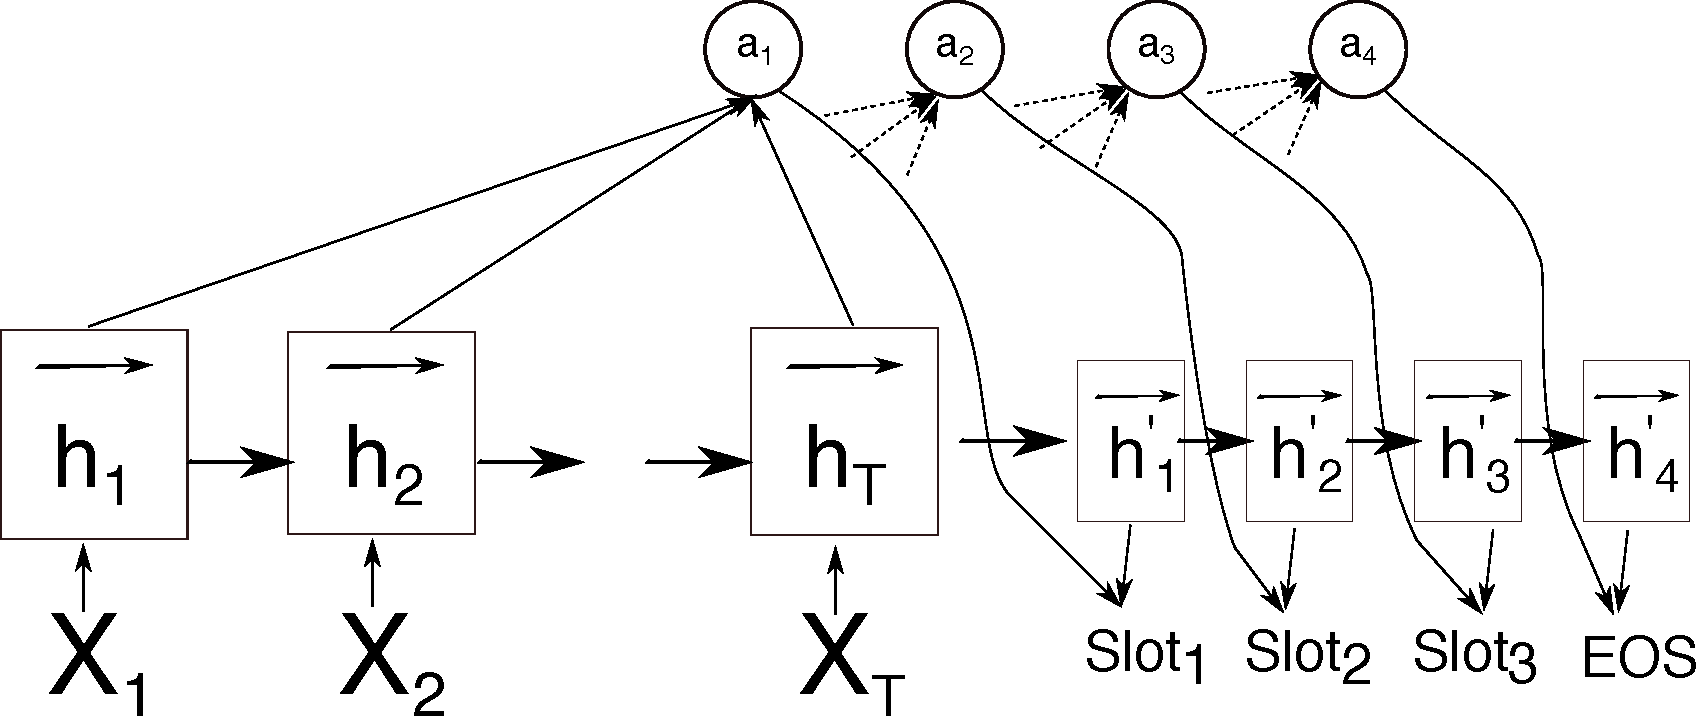
\includegraphics[width=0.7\textwidth]{encdec}
    \end{center}
\end{frame}

\begin{frame}\frametitle{Dialogue state tracking (DST) results}
\begin{center}
% 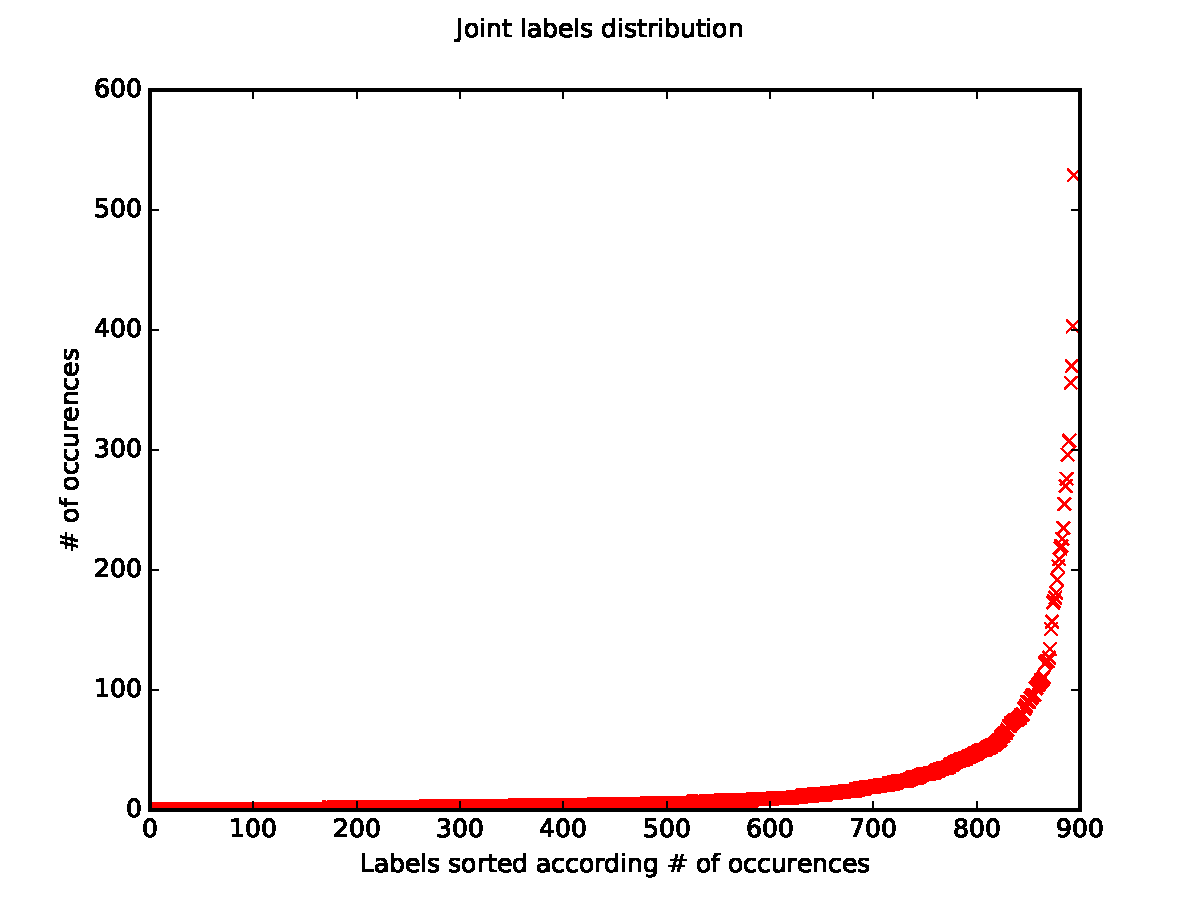
\includegraphics[width=0.6\textwidth]{jointLabelsDistrib} \\
\includegraphics[width=0.3\textwidth]{DB_features.png} \\
\begin{tabular}{l@{\quad}rll}
\hline
\multicolumn{1}{l}{\rule{0pt}{12pt}
                   {\it Model}}&\multicolumn{1}{l}{\it Dev set}&\multicolumn{2}{l}{\it Test set}\\[2pt]
\hline\rule{0pt}{12pt}
    {\bf \citet{platek2016recurrent} -- EncDec} &   0.867 & 0.730 \\
\hline
    \citet{vodolan_hybrid_2015} & - & 0.745 \\
    \citet{zilka_incremental_2015} & 0.69 & 0.72 \\
    \citet{henderson2013deep} & - & 0.737 \\
\hline
    DSTC2 stacking ensemble~\cite{henderson2014second} & - & 0.789 \\
\hline
\end{tabular}
\end{center}
\end{frame}

\begin{frame}\frametitle{DST is it necessary?}
    \begin{itemize}
        \item Representation used for KB query and response generation
        \item Training feasible only supervised manner
        \begin{itemize}
            \item reinforcement signal would be very weak
        \end{itemize}
        \item Labels defined based on handcrafted ontology
        \begin{itemize}
            \item Hard task for crowd-source workers
        \end{itemize}
        \item Action selection as well KB response may be obtained directly (work in progress)
    \end{itemize}
\end{frame}

% TODO backup slide complicated model which I discarded

\begin{frame}\frametitle{Data collection of simplified}
\end{frame}

\section{Research directions}  %%%%%%%%%%%%%%%%%%%%%%%%%%%%%%%%%%%%%%%%%%%%%%%%%%%%%%%%%%%%%%%%

\subsection{End-to-end optimized conversational model}
\begin{frame}\frametitle{State of end-end optimization}
\end{frame}

\subsection{Data collection and wizard of Oz}



% \plain{The End\\Thank you!}

\appendix

\begin{frame}[allowframebreaks]
        \frametitle{References}
        \bibliographystyle{plainnat}
        \bibliography{literature.bib}
\end{frame}

\end{document}
